\subsection{Client}

The customer can interact easily with the application thanks to a graphical user
interface, implemented with \specialname{JavaFX} library, or he can use the
command line interface version (CLI). When the customer issues a command the
middleware will handle this \code{Request Message}, it will serialize it in an
XML document and send it to the remote server application, which will produce
and send back a \code{Response Message}. After the response is received from the
client the middleware will manage to forward to the upper layer (the GUI) the
data just retrieved in a proper format. In Figure~\ref{fig:client} we can see
the UML implementation diagram of the Client side of the application.

%TODO
\begin{landscape}
	\begin{figure}
		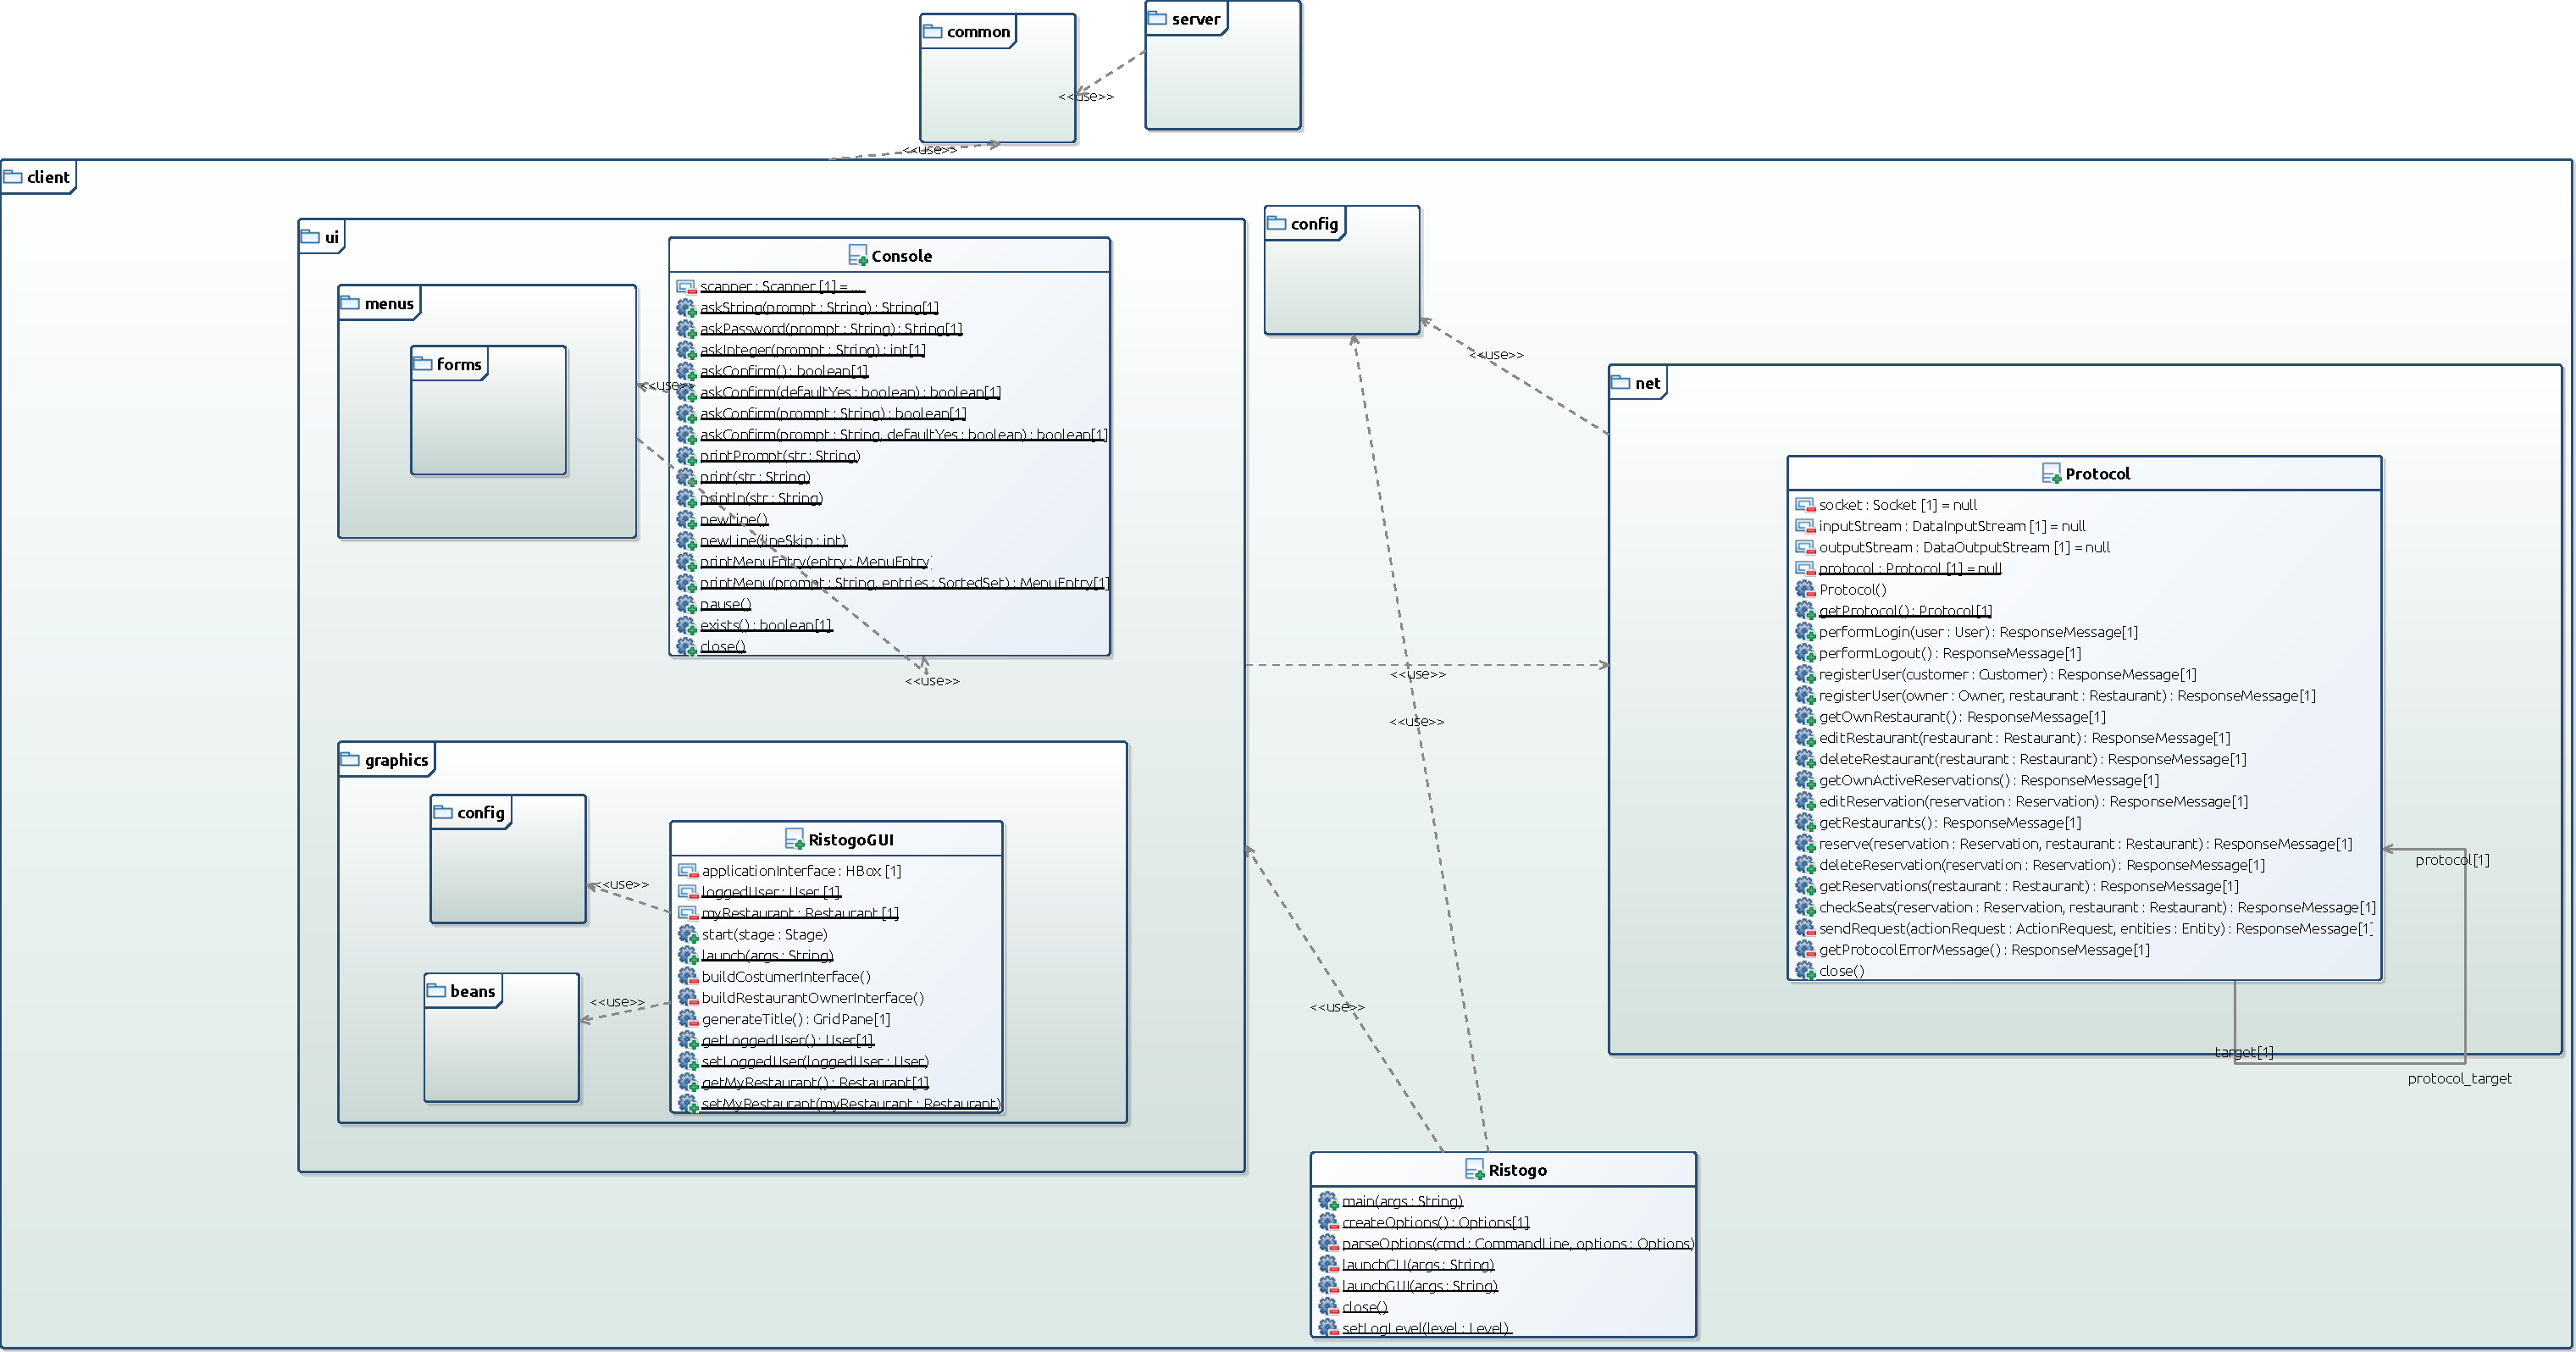
\includegraphics[width=0.85\paperheight]{client}
		\caption{\code{ristogo.client} UML Implementation Diagram.}
		\label{fig:client}
	\end{figure}
\end{landscape}
